%%%%%%%%%%%%%%%%%%%%%%%%%%%%%%%%%%%%%%%%%%%%%%%%%%%%%%%%%%%%%%%%%%%%%%%%%%%%%%%%%%%%%%%%%%%%%%%%%%%%%%%%%%%%%%%%%%%%%%%%%%%%%%%%%%%%%%%%%%%%%%%%%%%%%%%%%%%
% This is just an example/guide for you to refer to when submitting manuscripts to Frontiers, it is not mandatory to use Frontiers .cls files nor frontiers.tex  %
% This will only generate the Manuscript, the final article will be typeset by Frontiers after acceptance.   
%                                              %
%                                                                                                                                                         %
% When submitting your files, remember to upload this *tex file, the pdf generated with it, the *bib file (if bibliography is not within the *tex) and all the figures.
%%%%%%%%%%%%%%%%%%%%%%%%%%%%%%%%%%%%%%%%%%%%%%%%%%%%%%%%%%%%%%%%%%%%%%%%%%%%%%%%%%%%%%%%%%%%%%%%%%%%%%%%%%%%%%%%%%%%%%%%%%%%%%%%%%%%%%%%%%%%%%%%%%%%%%%%%%%

%%% Version 3.4 Generated 2018/06/15 %%%
%%% You will need to have the following packages installed: datetime, fmtcount, etoolbox, fcprefix, which are normally inlcuded in WinEdt. %%%
%%% In http://www.ctan.org/ you can find the packages and how to install them, if necessary. %%%
%%%  NB logo1.jpg is required in the path in order to correctly compile front page header %%%

\documentclass[utf8]{frontiersSCNS} % for Science, Engineering and Humanities and Social Sciences articles
%\documentclass[utf8]{frontiersHLTH} % for Health articles
%\documentclass[utf8]{frontiersFPHY} % for Physics and Applied Mathematics and Statistics articles

%\setcitestyle{square} % for Physics and Applied Mathematics and Statistics articles
\usepackage{url,hyperref,lineno,microtype,subcaption}
\usepackage[onehalfspacing]{setspace}
\usepackage[utf8]{vietnam}
\usepackage{hyperref}
%\linenumbers


% Leave a blank line between paragraphs instead of using \\


\def\keyFont{\fontsize{8}{11}\helveticabold }
\def\firstAuthorLast{22-03-2023} %use et al only if is more than 1 author
\def\Authors{Lê Thanh Nam\,$^{1,*, 2, 3, 4}$}
%\def\Authors{Lê Thanh Nam\,$^{1,*}$, Co-Author\,$^{2}$ and Co-Author\,$^{1,2}$}
% Affiliations should be keyed to the author's name with superscript numbers and be listed as follows: Laboratory, Institute, Department, Organization, City, State abbreviation (USA, Canada, Australia), and Country (without detailed address information such as city zip codes or street names).
% If one of the authors has a change of address, list the new address below the correspondence details using a superscript symbol and use the same symbol to indicate the author in the author list.
\def\Address{$^{1}$Tiến Sĩ, Kĩ Sư Xây Dựng: Viện Đô Thị Thông Minh và Quản Lý (ISCM), Trường Công Nghệ và Thiết Kế, Đại Học UEH, tp. Hồ Chí Minh -  \href{https://www.iscm.ueh.edu.vn/}{www.iscm.ueh.edu.vn} \\
$^{2}$Giám Đốc Kĩ Thuật, Chuyên Gia Soạn Hợp Đồng (FIDIC): Công Ty Tư Vấn ARCADIS, phụ trách thị trường Đông Nam Á và Ấn Độ -  \href{www.arcadis.com}{www.arcadis.com}\\
$^{3}$Giám Đốc: Công ty TNHH ASQ Việt Nam - \href{https://www.asq.vn}{www.asq.vn}\\
$^{4}$Cố Vấn Kĩ Thuật: Công ty EMAPTA - \href{www.emapta.com}{www.emapta.com}}
% The Corresponding Author should be marked with an asterisk
% Provide the exact contact address (this time including street name and city zip code) and email of the corresponding author
\def\corrAuthor{Di Động: +84-9-8378-0100 (Việt Nam) / +91-98-1044-4723 (Ấn Độ) Email: namlt@ueh.edu.vn}

%\def\corrEmail{Email: namlt@ueh.edu.vn}




\begin{document}
\onecolumn
\firstpage{1}

\title[Ứng Dụng Dữ Liệu Lớn/Quản Lý Hạ Tầng - Điện Lực]{Ứng Dụng Dữ Liệu Lớn và Quản Lý Tài Sản Hạ Tầng Trong Ngành Điện Lực} 

\author[\firstAuthorLast ]{\Authors} %This field will be automatically populated
\address{} %This field will be automatically populated
\correspondance{} %This field will be automatically populated

\extraAuth{}% If there are more than 1 corresponding author, comment this line and uncomment the next one.
%\extraAuth{corresponding Author2 \\ Laboratory X2, Institute X2, Department X2, Organization X2, Street X2, City X2 , State XX2 (only USA, Canada and Australia), Zip Code2, X2 Country X2, email2@uni2.edu}


\maketitle


\begin{abstract}
%Bài viết này tổng hợp 
Ngành điện lực là một trong những ngành xương sống cho sự phát triển kinh tế của quốc gia. Trong những năm gần đây, các công ty điện lực đã chứng kiến và trải nghiệm nhiều thử thách và sự đổi mới trong cả kĩ thuật và quản lý, và phần nào đã có những bước tiến đáng kể trong công tác chuyển đổi số (digitization) cùng với khái niệm về hệ thống truyền tải điện thông minh(Smart Grids). Các hệ thống điện thường luôn hoạt động trong tình trạng áp lực, chủ yếu là do sự gia tăng hàng năm trong nhu cầu sử dụng điện, sự thiếu hụt về nguồn cung về nhiên liệu/năng lượng để sản xuất ra điện, và các ràng buộc về môi trường áp đặt lên hệ thống sản xuất điện và sự mở rộng các đường dây tải điện. 

Ở Việt Nam, tổng công ty điện lực Việt Nam (EVN) cùng các bộ ngành liên quan đã soạn thảo và đề xuất "Qui Hoạch Điện VIII" hướng tới sự phát triển ổn định và bền vững chiến lược đến năm 2050. Một trong những nội dung quan trọng của Qui Điện VIII có chú trọng đến việc phát triển và nâng cao khả năng ứng dụng các công nghệ tiên tiến và áp dụng dữ liệu lớn cũng như trí thông minh nhân tạo vào công tác xây dựng, điều hành và quản lý các hệ thống điện.

Bài viết này cung cấp cho người đọc một cái nhìn tổng quan về các ứng dụng phân tích dữ liệu lớn, công tác quản lý cơ sở hạ tầng trong ngành điện lực, và các vấn đề liên quan đến việc triển khai. Chú trọng của bài viết sẽ là các ứng dụng mới đã mang lại giá trị tích cực trong ngành, một số bài học rút ra từ việc triển khai ứng dụng tại một số tổ chức, và một số ý tưởng và chủ đề cần khám phá. Tổng quan các nghiên cứu khoa học trong ngành khoa học dữ liệu trong ngành điện sẽ được đề cập nhằm tạo ra được cái nhìn tổng quát cho việc ứng dụng và tiếp tục phát triển của ngành trong tương lai. Cuối cùng, bài viết nêu ra các cơ hội và thách thức cũng như các mục tiêu và chiến lược để đạt được các kết quả có ý nghĩa.


%Bài viết này chú trọng đến vài trò của công tác phân tích dữ liệu lớn và vai trò của công tác quản lý cơ sở hạ tầng trong các lĩnh vực quan trọng của nền kinh tế, đặc biệt chú trọng tới ngành điện. Nội dung bài viết đề cập đến việc sử dụng các nguồn cung cấp dữ liệu lớn mà rất khó có thể truy cập vào các hệ thống cơ sở dữ liệu tiêu chuẩn, việc quản lý và quan trắc trong ngành điện. Đảm bảo sự ổn định của hệ thống thông qua việc sử dụng hiệu quả các nguồn dữ liệu lớn là một trong những mục tiêu quan trọng của các công ty điện lực.


\tiny
 \keyFont{ \section{Từ Khóa:} Dữ Liệu Lớn, Quản Lý Tài Sản, Cơ Sở Hạ Tầng, Độ Tin Cậy, Trí Thông Minh Nhân Tạo} %All article types: you may provide up to 8 keywords; at least 5 are mandatory.
\end{abstract}

\section{Giới Thiệu}
%For Original Research Articles \citep{conference}, Clinical Trial Articles \citep{article}, and Technology Reports \citep{patent}, the introduction should be succinct, with no subheadings \citep{book}. For Case Reports the Introduction should include symptoms at presentation \citep{chapter}, physical exams and lab results \citep{dataset}.

Có rất nhiều định nghĩa và cách hiểu khác nhau về phân tích dữ liệu lớn trong các ứng dụng ngành điện, đặc biệt là công tác sản xuất, truyền tải, và phân phối. Điều này chủ yếu là vì lý do có khá nhiều cách tiếp cận trong ngành khoa học dữ liệu và mục đích rộng liên quan (ví dụ như việc sử dụng các công cụ toán xác xác thống kê, trí thông minh nhân tạo (AI), học máy). Tính phức tạp và đa dạng của phân tích dữ liệu lớn trong ngành còn đến từ nhiều cách thức ứng dụng trong các lĩnh vực như quản lý tài sản (Asset Management), điều hành, điều khiển hệ thống, an toàn và an ninh, các quyết định lập kế hoạch và thị trường. Trong đó, có một vấn đề nền tảng làm cho công tác phân tích dữ liệu lớn trong ngành điện lực đặc biệt khó khăn là liên quan đến dung lượng của dữ liệu. Dung lượng của dữ liệu trong ngành thường ở cấp độ Terabyte, lớn hơn rất nhiều cấp độ Petabyte là cấp độ đã được coi là lớn trong các lĩnh vực khác. Cuối cùng, khái niệm "phân tích dữ liệu" còn là khá mơ hồ và đôi khi bị hiểu sai bởi vì hầu hết các ứng dựng cơ bản hay ứng dụng truyền thống trong ngành điện là dựa trên việc xử lý các dữ liệu được đo đạc (measurement data). Công việc xử lý truyền thống này đôi khi không được coi là phân tích dữ liệu lớn trong ngành khoa học dữ liệu. Ví dụ như, các phương pháp truyền thống liên quan đến tính toán ước lượng trạng thái (state estimation) hay vị trí sự cố (outage location) thường không được coi là phân tích dữ liệu lớn nếu công tác phân tích này chỉ đơn thuần dựa vào các phương trình/công thức toán được phát triển trên nền tảng vật lý. Trong khi đó, ở một khía cạnh khác, việc phán đoán sự cố dựa trên các mô hình nền tảng dữ liệu sử dụng các dữ liệu về thời tiết và mất điện có độ phân giải cao thì được coi là phân tích dữ liệu lớn.

Bài viết này không chú trọng đến việc đưa ra một định nghĩa rành mạch về phân tích dữ liệu lớn trong ngành điện mà chỉ chú trọng đến việc tổng quan hóa và nêu ra một số nghiên cứu và ứng dụng gần nhất sử dụng các phương pháp tiên tiến trong ngành khoa học dữ liệu trong ngành điện, đặc biệt chú trọng đến công tác quản lý tài sản cơ sở hạ tầng ngành điện, quản lý sự cố, và tính tích hợp với năng lượng tái tạo.

Có thể nói, một trong những bài báo nghiên cứu đầu tiên liên quan đến việc ứng dụng dữ liệu lớn trong ngành điện là bài báo của tác giả \cite{Kezunovic2013}. Tuy nhiên, nghiên cứu này chỉ dừng lại ở dạng mô hình và lý thuyết mà chưa đưa ra ứng dụng cụ thể vào thực tế. Việc ứng dụng vào thực tế mới chỉ được tiến hành trong vài năm gần đây.

Với mục đích hướng tới việc truyền tải kiến thức và đào tạo, ở bài viết này, một số khái niệm cơ bản cấu thành nên công tác phân tích dữ liệu lớn trong ngành điện và các khía cạnh đặc thù của ngành điện sẽ được đề cập. 

\section{Tầm Quan Trọng và Tính Khả Thi của Phân Tích Dữ Liệu Lớn trong Ngành Điện}
\subsection{Sự Tác Động của Phân Tích Dữ Liệu Lớn}

Sự thay đổi mạnh mẽ trong ngành điện dường như là chưa có tiền lệ, bao gồm sự chuyển dịch trong phân bổ tỷ lệ các dạng năng lượng (Energy Mix), yêu cầu và nhu cầu ngành càng cao của khách hàng, sự xuất hiện các kĩ thuật tiên tiến và thiết bị mới, và các mô hình kinh doanh mới. Chính những thay đổi này dẫn đến tính phức tạp (Complexity) và tính không chắc chắn (Uncertainty), cũng như mang tới các thách thức và cơ hội mới. Ở trung tâm của việc giải quyết các thách thức chính là việc đưa ra các quyết định tốt hơn và tối ưu hơn trong giai đoạn vận hành và lập kế hoạch, bao gồm cả công tác đầu tư dài hạn và phát triển chính sách.

Như chúng ta đã biết, lưới điện thông minh ngày này đã và đang tiếp tục được trang bị các thiết bị có khả năng cảm biến (sensing) và thu thập dữ liệu với độ phân giải cao hơn nhiều so với trước đây. Dữ liệu mới kèm theo các phương pháp phân tích mới có thể hỗ trợ các mục tiêu trong quản lý hệ thống điện như việc đạt được độ bền cao hơn, hiệu quả kinh tế tốt hơn và giảm khí thải. 

Phân tích dữ liệu vì thế trở thành một trong những yếu tố quan trọng giúp phần đảm bảo và nâng cao các công nghệ hiện có nhằm đưa ra các quyết định tối ưu hơn. Có thể nói, công việc phân tích dữ liệu đã và đang trở thành khả năng cơ bản và lợi thế chiến lượng cho các tổ chức muốn đổi mới và luôn hướng tới việc cung cấp dịch vụ chất lượng tốt hơn cho khách hàng. Các ứng dụng của phân tích dữ liệu cho ngành điện là rất nhiều và có thể được xác định trong nhiều hoạt động của ngành. Do đó, phân tích dữ liệu lớn đã, đang và sẽ là một bước đổi mới quan trọng trong đối trong các tổ chức cơ quan ngành điện lực.

\subsection{Các Nguồn Dữ Liệu Mới}
Việc áp dụng các giải pháp phân tích dữ liệu lớn trong các hệ thống phân phối và truyền tải điện khác nhau thường được tập trung vào việc khai thác các nguồn dữ liệu hỗn hợp (heterogeneous), là các khối dữ liệu có chất lượng riêng biệt, độ phân giải không gian/và thời gian khách nhau, và có cách trình bày thông tin khác nhau. Sẽ là khả thi để nâng cao ứng dụng nguồn dữ liệu này thông qua các phương pháp như: (a) kết hợp các nguồn dữ liệu mới và nguồn dữ liệu truyền thống, ví dụ thông qua việc sử dụng lý thuyết hợp nhất dữ liệu (data fusion) \citep{SimoesCosta2013}; (b) trích xuất và kết hợp thông tin từ các dữ liệu có định dạng khác nhau (ví dụ như dữ liệu ở hạng ảnh và ở dạng văn bản) thông qua các mô hình đã chiều (multimodal learning) \citep{Srivastava2012} hoặc qua một mạng lưới thông tin hỗ hợp (heterogeneous) \citep{Sun2016}; và (c) kết hợp dữ liệu từ các nguồn dữ liệu phân tán về mặt địa lý, ví dụ như việc sử dụng các phương pháp vector autoregressive (VAR) truyền thống \citep{Cavalcante2017} hay phương pháp học sâu (deep learning) \citep{Zhu2020}.

Các nguồn dữ liệu mới đến từ các lĩnh vực khác nhau:

\begin{itemize}
	\item \textbf{Hạ tầng mạng lưới điện}: Các cơ quan quản lý và điều hành hệ thống đang cải thiện và nâng cao khả năng quan sát của hệ thống mạng bằng cách lắp đặt các đơn vị đo pha (PMU) có thể cung cấp dữ liệu với tốc độ báo cáo cao (ví dụ, 30 đơn vị đo lường trên mỗi giây của độ lớn điện áp/dòng điện, pha và tần số) và các thiết bị đầu cuối điểm từ xa (Remote Terminal Units - RTU) tại các trạm biến áp và các công tơ điện thông minh lắp đặt cho khách hàng. Các cảm biến được dùng cho việc giám sát từ xa các trạm biến áp cũng đang được thử nghiệm để theo dõi tình trạng làm việc của thiết bị và cải thiện chất lượng dịch vụ \citep{Leitao2015}.
	
	\item \textbf{Các nhà máy điện tái tạo}: Công nghiệp năng lượng tái tạo đang lắp đặt và vận hành các cảm biến giám sát tại cấp độ cánh quạt điện gió và tấm năng lượng mặt trời, tạo ra một lượng lớn dữ liệu (ví dụ, một cánh quạt điện gió có thể có hơn 100 cảm biến bên trong cánh quạt, thu thập hơn 10.000 điểm dữ liệu mỗi giây) có thể được sử dụng cho việc bảo trì dự đoán (và giảm chi phí Vận hành và Bảo trì); dữ liệu từ một lưới dự báo thời tiết số, các cảm biến phân tán địa lý (ví dụ, cánh quạt điện gió, các cảm biến đo độ chiếu sáng), máy ảnh ghi lại bầu trời và hình ảnh vệ tinh có thể được kết hợp để cải thiện khả năng dự báo công suất (và thời tiết) trong nhiều khung thời gian khác nhau \citep{Sweeney2020}. Trong việc dự báo điện năng tái tạo, quy mô của các nghiên cứu cũng đã tăng từ một địa điểm đến hơn 100 địa điểm \citep{Messner2019}.
	
	\item \textbf{Người tiêu dùng và mạng xã hội}: trong khi đang ở giai đoạn đầu của triển khai, sự lan rộng của các thiết bị liên kết Internet trong các căn hộ và tòa nhà thông minh đang tạo điều kiện cho các dịch vụ về năng lượng và phi năng lượng dựa trên dữ liệu \citep{Ahmed2016}, ảnh hưởng của chúng phụ thuộc vào việc giải quyết các thách thức như bảo vệ/quyền riêng tư dữ liệu và tương tác với người tiêu dùng. Hơn nữa, sự gia tăng của mạng xã hội đã cho phép các công ty điện lực hiểu và tương tác với khách hàng tốt hơn bao giờ hết \citep{MorenoMunoz2016}. Các nhà nghiên cứu cũng đã thử kết hợp dữ liệu Twitter vào việc phát hiện cục bộ mất điện \citep{Sun2016}.
	
	\item \textbf{Thị trường điện}: Trong vài năm qua, đặc biệt tại châu Âu, tính minh bạch của thị trường điện đã được cải thiện đáng kể, và sau khi xuất bản Quy định (EU) số 5 43/2013 [22], lượng dữ liệu công khai có sẵn đang tăng lên [23], bao gồm cả truy cập vào các đề xuất riêng lẻ từ các công ty cung cấp điện trên thị trường (thông thường có sẵn với độ trễ vài tháng). Cùng xu hướng đó đang diễn ra ở Mỹ, với các nền tảng như bộ sưu tập dữ liệu Form EIA-930 cung cấp nguồn dữ liệu toàn diện và tập trung cho các dữ liệu hoạt động hàng giờ của lưới điện cao áp tại 48 tiểu bang. Dữ liệu mở này có thể được sử dụng cho các mục đích khác nhau: cải thiện kỹ năng dự báo giá điện bằng cách kết hợp phân tích giá điện từ các khu vực khác nhau [24] hoặc đánh giá ảnh hưởng quy mô lớn của việc phát điện từ nguồn năng lượng tái tạo được cấp bởi lưới điện liên kết với các quốc gia láng giềng [25].
	
	\item \textbf{Lĩnh vực môi trường và thời tiết}: Dữ liệu thời tiết đóng vai trò quan trọng trong việc dự đoán điều kiện hoạt động, bao gồm cả lỗi hỏng hóc thiết bị và đường dây. Dữ liệu từ các trạm thời tiết trên mặt đất [26], vệ tinh [27] và tài nguyên radar [28] có sẵn từ cơ sở dữ liệu của chính phủ. Mạng lưới cảm biến chuyên dụng, chẳng hạn như mạng lưới phát hiện sét quốc gia ở Mỹ [29], cũng là nguồn cung cấp dữ liệu thời tiết khá hữu ích. Nhiều dịch vụ dự báo thời tiết cũng có sẵn để cung cấp các tính năng được tính trước của các tập dữ liệu thời tiết [30]. Ngoài ra, dữ liệu về thực vật, đất đai, di cư động vật và các điều kiện xung quanh khác cũng có thể có sẵn từ nhiều nguồn khác nhau [31]. Cách sử dụng dữ liệu chính xác cao bằng cách sử dụng các cơ sở dữ liệu chuyên dụng như hệ thống (LIDAR - Light Detection and Ranging) hoặc khảo sát bằng thiết bị bay drone cũng được nghiên cứu và đưa vào thực tiễn [32]. Những dữ liệu này thường không được thu thập trong phạm vi chức năng của ngành điện nhưng chúng lại là một nguồn dữ liệu quan trọng cho ngành này. Chẳng hạn, trong dự báo tải, các nghiên cứu đã chuyển từ việc sử dụng nhiệt độ được thu thập tại một trạm đến nhiều biến thời tiết và nhiều trạm thời tiết [33-35]. Trong dự báo điện mặt trời, dữ liệu hình ảnh bầu trời được sử dụng nhiều để phát hiện đám mây [36].
\end{itemize}

Các nhà nghiên cứu và chuyên gia hiện nay tập trung vào việc khai thác dữ liệu hiện có và khám phá các nguồn dữ liệu mới nổi và dữ liệu với quy mô lớn để theo đuổi các cải tiến trong kế hoạch và vận hành lưới điện. Có nhiều khía cạnh quan trọng khác của phân tích dữ liệu lớn, chẳng hạn như xây dựng thuật toán có thể tận dụng môi trường tính toán hiệu suất cao và mở rộng kích thước mô hình để nắm bắt các đặc trưng chi tiết trong dữ liệu [37]. Một ví dụ khác là sử dụng dữ liệu tải và thời tiết hàng giờ để dự báo tải dài hạn, thông thường dựa trên dữ liệu hàng tháng [38,39]. Một bài đánh giá gần đây về phân tích dữ liệu lấy từ các công tơ thông minh liệt kê 10 bộ dữ liệu công khai về nhu cầu điện [40]. Hình \ref{fig:1} là một ví dụ mô tả các thuộc tính cơ bản của dữ liệu lớn trong ngành điện.

\begin{figure}[h!]
\centering
	\begin{center}
		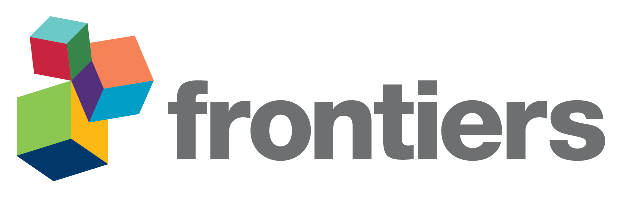
\includegraphics[width=10cm]{logo1}% This is a *.eps file
	\end{center}
	\caption{ Các thuộc tính cơ bản của dữ liệu lớn trong ngành điện}\label{fig:1}
\end{figure}


\subsection{Các Cân Nhắc Quan Trọng Khi Tạo Ra Các Tập Dữ Liệu}

Cách tạo các tập dữ liệu như thế nào là khá quan trọng để sử dụng và ứng dụng các công cụ phân tích dữ liệu lớn. Một số cân nhắc sau cần được quan tâm khi thiết lập, tạo lập, và thu thập các gói dữ liệu: 

\begin{itemize}
\item Tính đồng bộ và mối tương quan theo không gian và thời gian
\item Tính mở rộng
\item Dữ liệu trống
\item Sự đa dạng của dữ liệu xấu
\item Các loại dữ liệu có độ tin cậy thấp/có tính biến thiên cao
\end{itemize}

Cách mà mỗi yếu tố này phản ánh lên các ứng dụng dữ liệu lớn trong lưới điện nằm ngoài phạm vi của bài viết này, nhưng chắc chắn đáng khám phá khi các tập dữ liệu mới được thêm vào và kết hợp với nhau trong quá trình xử lý và phân tích.

\section{Thách Thức của Công Việc Phân Tích Dữ Liệu Lớn}
\subsection{Nền Tảng của Khoa Học Dữ Liệu}
Mục tiêu của khoa học dữ liệu là trích xuất giá trị từ dữ liệu. Các bước của vòng đời quản lý dữ liệu bao gồm thu thập dữ liệu; tiền xử lý (khám phá, lấy mẫu, giảm chiều/thu gọn các đặc trưng và thuộc tính, tạo đặc trưng và thuộc tính, biến đổi, làm sạch và tích hợp); xử lý phân tích (mô hình hóa, thường bao gồm nhiều khối mô hình xây dựng liên kết với nhau); giải thích và báo cáo kết quả [61]. Những kỹ năng chính cần thiết trong lĩnh vực này thường được xem là đa ngành ở giao điểm của khoa học máy tính, toán học, thống kê và các lãnh vực khoa học kĩ thuật và xã hội khác. Trên mặt kỹ thuật, các thách thức chính thường liên quan đến dữ liệu lớn, trí thông minh nhân tạo và các phương pháp học máy, trong khi quá trình khoa học dữ liệu áp dụng cũng có thể yêu cầu các kỹ năng khoa học xã hội, giao tiếp và kinh doanh. 

Một cái nhìn toàn diện về khoa học dữ liệu nhấn mạnh rằng khoa học dữ liệu là "hơn là sự kết hợp của thống kê và khoa học máy tính" vì "nó yêu cầu đào tạo làm sao để tổng hợp và kết nối giữa các kĩ thuật thống kê và sức mạnh của máy tính trong một khung làm việc lớn hơn, giải quyết từng vấn đề một cũng như giải quyết các câu hỏi cụ thể trong từng lĩnh vực". Các nhà nghiên cứu cũng có cùng quan điểm cho rằng ngành khoa học dữ liệu đòi hỏi: (1) hiểu về bối cảnh của dữ liệu, (2) đánh giá các trách nhiệm liên quan đến việc sử dụng dữ liệu riêng tư và công khai; và (3) giao tiếp rõ ràng về những gì có thể và không thể được suy ra từ một bộ dữ liệu.

Các thành phần cốt lõi của khoa học dữ liệu là các phương pháp dựa trên học máy (Machine Learning - ML) để tìm kiếm các khuôn mẫu (pattern) trong dữ liệu và dựa vào đó để cung cấp thông tin về hiện tượng được mô tả bởi dữ liệu và các dự đoán liên quan đến các sự kiện trong tương lai. Trong học máy , mục tiêu là học/tạo ra một hàm (ánh xạ) mô tả và chứa đựng các dự liệu đầu vào (thường gọi là các biến giải thích - explanatory variable) với tham số đầu ra quan sát được (gọi là biến phản ứng). Một biểu diễn đơn giản hóa của thực tế được tạo ra cho mục đích này, gọi là mô hình, được sử dụng để ước tính phản ứng chưa biết cho các trường hợp mới dựa trên các biến giải thích quan sát được quan tâm, và quá trình này được gọi là suy luận hoặc đơn giản hơn là dự đoán.

Các mục tiêu của học máy thường được nhóm thành các nhiệm vụ mô tả và nhiệm vụ dự đoán. Các nhiệm vụ mô tả nhằm khám phá các mô hình có thể diễn giải được mô tả dữ liệu trong quá khứ, và các nhiệm vụ dự đoán là những nhiệm vụ mà mục tiêu là xác định các mô hình được quan sát trong dữ liệu huấn luyện để ước tính các dự đoán về các rủi ro và các kết quả khác trong tương lai. Các nhiệm vụ mô tả thường là không giám sát, có nghĩa là chỉ các biến giải thích được xem xét trong phân tích. Các mục tiêu mô tả phổ biến bao gồm phân cụm dữ liệu [64,65], khám phá mối liên hệ [66], và phát hiện sự khác biệt so với hành vi bình thường, bao gồm phân tích giá trị cực đại, phát hiện giá trị ngoại lệ và xác định các mô hình mới nổi [67]. Các nhiệm vụ dự đoán là giám sát, có nghĩa là chúng không chỉ yêu cầu các biến giải thích mà còn giá trị của biến phụ thuộc đang được dự đoán. Các ví dụ thực tế bao gồm đánh giá rủi ro [68] và chẩn đoán bệnh [69].

Có các phương pháp bán giám sát [70] và tự đào tạo [71], trong đó dữ liệu huấn luyện bao gồm một số dữ liệu có nhãn và nhiều dữ liệu không có nhãn.

Trong phân loại, các biến phản hồi được dự đoán là một lớp (ví dụ, một trong vài loại nhãn dữ liệu), hoặc trong trường hợp hồi quy, đó là một giá trị liên tục. Một trong những phương pháp thường được sử dụng cho phân loại là cây quyết định (decision tree). Thuật toán Hunt [67], một trong những phương pháp cây quyết định sớm nhất, đề xuất quy trình tổng quát của việc phân chia dữ liệu dựa trên giá trị của một thuộc tính duy nhất và tiếp tục đệ quy trên các tập con nếu lớp không đủ thuần khiết ở các tập con. Nhiều phương pháp đã được đề xuất để đo độ không thuần khiết của tập dữ liệu và xác định phân nhánh tiếp theo (ví dụ: entropy trong CART [72] hoặc chỉ số Gini trong ID3 [73] và C4.5 [74]), cũng như để tỉa cây, từ đó cải thiện khả năng tổng quát của mô hình. Cây quyết định dễ hiểu, rất rẻ để xây dựng và rất nhanh trong việc phân loại các trường hợp không rõ ràng. Chúng cũng khá bền với nhiễu và có thể xử lý các thuộc tính trùng lặp hoặc không liên quan, nhưng không tính đến sự tương tác giữa các thuộc tính. Một trong những hạn chế của cây quyết định là chúng yêu cầu tỉa, nếu không chúng sẽ trở nên quá lớn dẫn đến các vấn đề quá khớp. Giới hạn này được giải quyết thành công bằng Random Forests, được xây dựng như một tập hợp các cây quyết định không tương quan [75,76]. Tập hợp này được lấy cảm hứng từ phương pháp Bagging, một phương pháp tổng hợp dựa trên lấy mẫu bootstrap, được phát triển để giảm phương sai mà không làm tăng sai số [77]. Trong Random Forests, ý tưởng này được mở rộng hơn nữa bằng cách giới hạn mỗi nút chỉ xem xét một tập con ngẫu nhiên nhỏ của các thuộc tính. Giải pháp kết quả được chứng minh là chính xác hơn so với thuật toán AdaBoost.

Một kỹ thuật thay thế phổ biến có thể xử lý các tương tác giữa các biến giải thích là phân loại một trường hợp mới bằng cách tính khoảng cách đến k láng giềng gần nhất trong tập huấn luyện và dự đoán lớp dựa trên đa số hoặc đa số có trọng số của các láng giềng được xác định kết quả của chúng. Đây là một phương pháp học lười vì mô hình không được xây dựng rõ ràng và thời gian suy luận cần thiết để phân loại một trường hợp mới khá lớn. Nó cũng yêu cầu so sánh mỗi điểm dữ liệu mới với mỗi điểm dữ liệu trong tập huấn luyện. Ngoài ra, kỹ thuật này không dễ sử dụng khi nhiều giá trị thuộc tính bị thiếu, vì trong những trường hợp như vậy, phương pháp dựa trên khoảng cách để xác định láng giềng gần nhất có thể không đáng tin cậy. Một số trong số những giới hạn này có thể được vượt qua bằng cách sử dụng đồ thị gần nhất, trong đó các nút được kết nối nếu các điều kiện hình học nhất định được đáp ứng. Trong một công thức như vậy, các thuật toán đồ thị hiệu quả khác nhau (ví dụ: cây khung nhỏ nhất và tam giác hóa) có thể được sử dụng để xác định láng giềng gần nhất và tương quan hơn [80].

Một phương pháp phân loại thay thế toán học nghiêm ngặt hơn là ước tính xác suất hậu nghiệm của lớp mục tiêu bằng cách sử dụng định lý Bayes. Một phương pháp đơn giản nhưng thanh lịch và mạnh mẽ, được gọi là Naive Bayes, giả định rằng các giá trị thuộc tính độc lập có điều kiện với nhau, cho trước nhãn lớp y. Trong trường hợp như vậy, xác suất có điều kiện của lớp của tất cả các thuộc tính có thể được phân tách thành tích của xác suất có điều kiện của mỗi thuộc tính. Phương pháp này chống lại nhiễu, giá trị bị thiếu và các thuộc tính không liên quan. Tuy nhiên, sự độc lập có điều kiện giữa các biến giải thích là một giả định mạnh mẽ không hợp lệ trong nhiều ứng dụng. Đối với các kịch bản như vậy, một lớp mô hình đồ thị xác suất được gọi là Mạng tin cậy Bayesian đã được phát triển bằng cách mô hình hóa các phụ thuộc có điều kiện thông qua các đồ thị vô hướng có hướng. Sự suy luận chính xác trên các đồ thị như vậy là NP-khó [81], do đó, các ứng dụng của chúng bị giới hạn cho số lượng thuộc tính nhỏ hơn hoặc cho các loại cấu trúc đồ thị đặc biệt.

Một bộ phân loại xác suất hiệu quả khác là hồi quy logistic [82]. Chúng tôi đã thành công trong việc sử dụng phương pháp này để dự đoán xác suất mất điện liên quan đến thời tiết [83]. Giả sử một vấn đề hai lớp (phản hồi y = 0 hoặc 1), phương pháp này tránh việc ước tính trực tiếp xác suất có điều kiện của một trường hợp, mà thay vào đó ước tính tỷ lệ giữa xác suất lớp hậu nghiệm P(y=1|x)/P(y=0|x). Một lợi thế lớn của hồi quy logistic so với k láng giềng gần nhất là nó có thể áp dụng cho các vấn đề có số chiều cao, vì phương pháp không phụ thuộc vào việc đo đạc sự tương đồng giữa các điểm dữ liệu. Lợi ích khác của phương pháp này là các tham số trọng lượng tương ứng với các thuộc tính riêng lẻ và do đó cung cấp tính giải thích khá dễ dàng. Tuy nhiên, sự hiện diện của một số lượng lớn các thuộc tính không liên quan là một thách thức đối với hồi quy logistic, và phương pháp này không áp dụng cho việc phân loại các trường hợp với giá trị bị thiếu, điều này có thể là một hạn chế nghiêm trọng trong thực tế.

Mô hình hồi quy logistic có thể được xem như một trường hợp của mô hình tuyến tính tổng quát. Các mô hình mạnh mẽ khác trong danh mục này là Máy vector hỗ trợ (SVM) và Mạng neural đa tầng (MNN). Trong SVM, vấn đề tối ưu hóa được định hình như tìm kiếm ranh giới lớn nhất phân tách siêu mặt phẳng cho một khu vực lớn tồn tại ở mỗi bên của ranh giới quyết định [84]. Điều này được định hình như một vấn đề lập trình phi tuyến tính bị ràng buộc được biểu thị dưới dạng một hàm của các hệ số của siêu mặt phẳng phân tách, được giải quyết bằng phương pháp bội số Lagrange. Đối với phân loại phi tuyến tính, dữ liệu được chuyển đổi một cách ngầm định thành không gian có số chiều cao, nơi vấn đề có thể được phân tách tuyến tính. Điều này được đạt được bằng cách sử dụng kernel trick, để giảm bớt vấn đề hiệu quả thành tình huống phân loại tuyến tính. Sử dụng các kernel được chọn cẩn thận (Gaussian, đa thức hoặc sigmoid) cho phép xấp xỉ các ranh giới quyết định tùy ý. Các lợi ích chính của phương pháp SVM là nó chống lại nhiễu và giảm thiểu quá khớp trong khi tìm kiếm giá trị nhỏ nhất toàn cục của hàm mục tiêu. Tuy nhiên, chi phí tính toán của SVM là cao, và vẫn là một thách thức để sử dụng mô hình này khi các biến mô tả bị thiếu một phần trong dữ liệu quan sát.

Mạng nơ-ron tiến thẳng đa tầng (FNN) cũng được sử dụng thành công cho phân loại trong nhiều ứng dụng thách thức khác nhau [85]. Ví dụ, chúng tôi đã thành công trong việc huấn luyện FNN để phân biệt giữa dòng vào từ biến áp và dòng lỗi [86]. Mô hình này có ít nhất một lớp đơn vị ẩn, mỗi lớp tính toán một hàm phi tuyến mượt và khả vi của tổng đầu vào có trọng số (ví dụ, hàm sigmoid). Trong mô hình này, vấn đề cập nhật các tham số khi phát hiện lỗi ở đầu ra thường được giải quyết bằng cách truyền ngược lỗi từ đầu ra về các lớp trước đó. Trong quá trình này, lỗi của một nút trong lớp ẩn được ước tính dưới dạng một hàm của các ước tính lỗi và trọng số trong các nút trong lớp trước đó, và giá trị này được sử dụng để cập nhật trọng số của nút ẩn này bằng cách tính toán độ dốc lỗi đối với các trọng số trong nút [87]. FNN có thể xấp xỉ các hàm tùy ý, và do đó mạnh mẽ hơn SVM. Tuy nhiên, khi thiết kế một mạng, quá khớp phải được giải quyết cẩn thận. Ngoài ra, nhiễu trong dữ liệu có thể gây ra vấn đề huấn luyện, vì mô hình có thể hội tụ đến một cực tiểu cục bộ, và quá trình huấn luyện có thể yêu cầu một thời gian dài, giới hạn các ứng dụng thực tế. Vấn đề khác với FNN cổ điển là học các mạng sâu rất khó, do tác động kết hợp của việc bão hòa hàm kích hoạt sigmoid khi truyền ngược các lỗi nhỏ, dẫn đến sự hội tụ rất chậm. Tiến bộ lớn đã được đạt trong việc giải quyết vấn đề này, được gọi là vấn đề gradient biến mất, trong những năm gần đây. Điều này, cùng với tiến bộ trong cơ sở hạ tầng tính toán phân tán dựa trên GPU và sự có sẵn của các tập dữ liệu rất lớn, đã cho phép phát triển các mạng nơ-ron sâu hiệu quả, vượt trội hơn rất nhiều so với tất cả các phương pháp thách thức khác nhau, bao gồm thị giác máy tính, xử lý ngôn ngữ tự nhiên, phát âm.

Trong các hệ thống điện, dữ liệu thường được quan sát trên không gian và thời gian, và do đó, các phương pháp hồi quy cấu trúc dựa trên đồ thị tiên tiến hơn được sử dụng để khai thác các phụ thuộc cấu trúc. Ví dụ, chúng tôi đã sử dụng học có cấu trúc trong các trường ngẫu nhiên có điều kiện Gaussian để đánh giá rủi ro của sự phá vỡ cách điện cho một sự tiếp xúc cụ thể và các mối đe dọa thời tiết liên quan trong một mạng điện [91]. Nghiên cứu mới nhất về học sâu [88,92,93] cho thấy rằng một loạt các ứng dụng, bao gồm hồi quy cấu trúc, có thể được hưởng lợi từ việc học các biểu diễn tiềm ẩn cho dữ liệu đầu vào. Trong nghiên cứu của chúng tôi [94], việc học biểu diễn cho các trạm hệ thống điện, dựa trên sự gần nhau về không gian của chúng, đã rất có lợi cho việc dự đoán các lỗi cung cấp điện và ước tính xác suất lỗi cung cấp điện. Trong một phương pháp như vậy, các nút của đồ thị được nhúng trong không gian chiều thấp hơn, nơi các phương pháp học máy tiêu chuẩn có thể được áp dụng dễ dàng hơn. Các thuật toán nhúng nhằm giữ cấu trúc đồ thị và đơn giản hóa các mô hình học bằng cách di chuyển khỏi các biểu diễn đồ thị. Một lợi thế của việc sử dụng các phương pháp này là chúng có thể tiết lộ các phụ thuộc không gian phức tạp hơn có chứa một số tương tác xa hơn ngoài tác động của khu vực lân cận.

Quá trình nhúng nút đại diện cho đồ thị ban đầu trong một không gian đặc trưng mới, mô tả tốt nhất các mối quan hệ không gian của các nút trong đồ thị ban đầu. Đặc điểm này của quá trình nhúng nút nhằm bắt giữ các mối quan hệ cần thiết của cấu trúc đồ thị ban đầu trong khi đơn giản hóa biểu diễn thành một danh sách các vector đặc trưng chiều thấp hơn.

Có nhiều thuật toán để thu được nhúng như vậy; Hai thuật toán thường được sử dụng là DeepWalk [95] và Node2Vec [96]. Cả hai thuật toán đều dựa trên thông tin cộng đồng được thu được bằng các bước đi ngẫu nhiên, được sử dụng để học các biểu diễn không gian tiềm ẩn. Ngoài ra, DeepWalk có thể thực hiện khám phá cục bộ một cách hiệu quả và có thể chứa đựng các thay đổi nhỏ trong cấu trúc đồ thị mà không cần tính toán toàn cầu lại. Node2Vec là một khung công cụ thuật toán hóa mà tổng quát hóa quá trình DeepWalk để cung cấp một khái niệm linh hoạt về khu vực lân cận của một nút, cho phép học các biểu diễn phong phú hơn bằng cách khám phá hiệu quả các khu vực lân cận đa dạng. Giải pháp này đã được sử dụng thành công để phát triển một phương pháp mới cho dự báo bức xạ mặt trời, dựa trên các nhúng không gian và thời gian sử dụng mô hình Node2Vec cho dữ liệu đồ thị [97]. Phương pháp này đơn giản hóa các mô hình học bằng cách di chuyển khỏi các đồ thị phức tạp. Mô hình được phát triển cho các dự báo từ 3 đến 12 giờ. Mô hình đã dự đoán bức xạ mặt trời với độ chính xác rất cao vào mùa hè, khi có nhiều ngày trời quang đãng. Trong những tháng mùa đông, độ chính xác có một chút giảm, nhưng vẫn rất cao và vẫn mạnh mẽ ngay cả khi dữ liệu quan sát bị thiếu về mặt không gian và thời gian.


\subsection{Khía Cạnh Kĩ Thuật}
Trong khi phân tích dữ liệu lớn dựa trên nền tảng khoa học dữ liệu mạnh mẽ, cũng có một số khía cạnh quan trọng khác để các phương pháp đó được sử dụng trong thực tế. Khi tương tác với các chuyên gia và những người trong ngành cố gắng đạt được những lợi ích rõ ràng từ việc sử dụng khoa học dữ liệu, người ta thường nghe thấy rằng phần thực tế của khoa học dữ liệu có thể chỉ chiếm 10\% công việc, trong khi 90\% liên quan đến thiết lập quy trình làm việc, quản lý dữ liệu (và lưu trữ) cũng như các khía cạnh tính toán. Do đó, việc quan sát một số khía cạnh liên quan đến kỹ thuật trong phân tích dữ liệu lớn là rất quan trọng. Chúng đã được xác định là các thách thức chính cho sự thành công của phân tích dữ liệu lớn [98,99].

Ở trung tâm của khái niệm phân tích dữ liệu lớn là ý tưởng cơ bản rằng dữ liệu cần được xử lý là "lớn". Để định nghĩa đúng dữ liệu lớn và các tính năng cần thiết của nó, người đọc được giới thiệu đến [100]. Các ví dụ điển hình liên quan đến việc thu thập dữ liệu PMU, cũng như dữ liệu có độ phân giải cao ở mức tài sản, (ví dụ, từ các tuabin gió, bộ biến tần điện từ (PV), đồng hồ thông minh, v.v.). Tốc độ thu thập dữ liệu này ở các thang thời gian từ giây đến phút, và đồng thời ở nhiều vị trí địa lý khác nhau, trong khi cũng bao gồm nhiều loại biến số khác nhau. Nói chung, các dữ liệu như vậy trong lưới điện bao gồm các đo lường điểm, hình ảnh và có thể là văn bản. Một số khía cạnh của dữ liệu lớn này cho các hệ thống điện, từ thách thức đến ứng dụng, đã được Arghandeh và Zhou đề cập gần đây [9].

Trong hầu hết các tài liệu khoa học mô tả các ứng dụng điện và ngoài ra, được cho rằng dữ liệu có sẵn và chất lượng tốt. Tuy nhiên, bất kể khó khăn đến đâu, đảm bảo giao tiếp dữ liệu, đảm bảo tính toàn vẹn của dữ liệu, cũng như đảm bảo chất lượng dữ liệu, là các bước cần thiết trước khi thiết kế và triển khai một giải pháp dựa trên dữ liệu [101]. Ngược lại, những khía cạnh liên quan đến tính sẵn có và chất lượng dữ liệu đã được xem xét trong một thời gian khá lâu bởi cộng đồng khoa học máy tính, cho đó đề xuất một số phương pháp [102]. Sau đó, việc làm sạch dữ liệu và sửa đổi các bộ dữ liệu thường được liên quan đến, mặc dù người ta nên nhận thức rằng những hành động này thực sự có thể ảnh hưởng đến thông tin ban đầu trong các bộ dữ liệu, ví dụ như trong các thuộc tính thống kê của nó [103]. Đối với các ứng dụng trong các thị trường điện liên quan đến năng lượng tái tạo, một vấn đề cổ điển ví dụ là điền vào các khoảng trống trong chuỗi thời gian, tức là có thể có các khoảng thời gian mà dữ liệu đơn giản không có sẵn, do các lỗi trong việc đăng nhập, lưu trữ hoặc truyền dữ liệu. Để điền vào những khoảng trống này, đã đề xuất nhiều phương pháp, tận dụng dữ liệu xung quanh khoảng thời gian đó, dữ liệu với phụ thuộc không gian thời gian (đặc biệt liên quan đến việc tạo ra năng lượng tái tạo dựa trên thời tiết), tính sẵn có của dữ liệu ở các mức tổng hợp khác nhau, cũng như mối quan hệ vật lý giữa các biến số quan tâm (ví dụ, trong một vấn đề luồng điện tối ưu). Đối với một ví dụ gần đây liên quan đến dữ liệu tải điện, xem thảo luận trong [104].

Ngoài những khía cạnh liên quan đến dữ liệu, các phương pháp dựa trên dữ liệu được sử dụng trên các tập dữ liệu lớn đòi hỏi năng lực tính toán đáng kể để giải quyết các vấn đề mô phỏng và tối ưu hóa liên quan. Để tập trung dữ liệu, những vấn đề này có thể được giải quyết thông qua tính toán hiệu năng cao (HPC), ngày càng trở nên phổ biến trong các ứng dụng lưới điện và thị trường điện [105]. Những ví dụ đáng chú ý bao gồm luồng công suất tối ưu [106] và vấn đề chuyển mạch truyền tải [107]. Việc giải quyết các vấn đề quy mô lớn đó với HPC sẽ liên quan đến một số kỹ thuật phân rã, cũng trở nên phổ biến trong các vấn đề vận hành, thị trường và kế hoạch hệ thống điện [108]. Tuy nhiên, cũng có thể có một số ứng dụng mà điều này không phải là khả thi hoặc không muốn tập trung dữ liệu. Trong trường hợp đó, các phương pháp tương tự có thể được sử dụng để giải quyết các vấn đề này theo cách phi tập trung, tuy nhiên, có thể phải chịu gánh nặng giao tiếp tăng do tính chất lặp lại của các phương pháp tối ưu hóa phân tán. Những ví dụ đáng chú ý bao gồm các vấn đề luồng công suất tối ưu [109] và học phân tán cho dự báo năng lượng tái tạo [110]. Có lẽ trong tương lai, các thiết lập liên quan sẽ không được tập trung hoàn toàn hoặc phi tập trung hoàn toàn và sẽ phụ thuộc vào tính toán đám mây, fog và edge computing [111].

Phân tích dữ liệu lớn cần được đặt trong khung cảnh tổng thể của giải quyết vấn đề. Trong thực tế, đó chỉ là một công cụ bổ sung để hỗ trợ hoạt động và ra quyết định. Do đó, trước khi đầu tư vào các thiết lập dữ liệu lớn cụ thể và các công cụ phân tích, vấn đề và phương pháp giải quyết vấn đề liên quan cần được xác định rõ ràng. Ví dụ, nếu các dự báo được sử dụng để hỗ trợ ra quyết định, loại dự báo (ví dụ, xác định hoặc xác suất) và các sản phẩm dự báo (độ phân giải, chuẩn hóa, vv.) nên được quyết định dựa trên vấn đề quyết định cụ thể. Ngoài ra, khi chuyển từ dữ liệu sang phân tích, thường có nhu cầu cho một lớp trích xuất đúng loại và mức thông tin từ dữ liệu thô. Điều này có thể được thực hiện dựa trên bộ lọc và làm mịn, kỹ thuật kỹ thuật đặc trưng, vv. Một ví dụ điển hình sẽ là phát hiện sự kiện dựa trên các luồng dữ liệu, sau đó được sử dụng làm đầu vào cho một số vấn đề phân tích khác.

Các yêu cầu bổ sung có thể mang lại một cấp độ phức tạp khác cho phân tích dữ liệu lớn. Yêu cầu quan trọng liên quan đến dữ liệu chính nó (và các luồng dữ liệu liên quan) là cách xử lý an ninh mạng và quyền riêng tư trong lưới điện. Hiện nay, an ninh mạng đại diện cho một thành phần quan trọng của hệ thống năng lượng phân phối trong tương lai, mà trên đó phân tích dữ liệu lớn có thể được thực hiện [112]. Do đó, thiết lập cho phân tích dữ liệu lớn, cũng như các công cụ được sử dụng, cần phải mạnh mẽ để có thể chịu đựng được việc loại bỏ các dữ liệu quan trọng hoặc làm giả dữ liệu. Ngoài ra, quyền riêng tư dữ liệu đang trở thành mối quan tâm ngày càng tăng vì nếu dữ liệu đang được thu thập được chia sẻ, có thể suy ra thông tin về các tài sản hoặc người tiêu dùng cụ thể, điều đó không hề được định sẵn. Mối quan tâm về quyền riêng tư đặc biệt hiện nay khi các đồng hồ đo thông minh được triển khai rộng rãi [113], cho phép một số người có thể có thông tin về thói quen tiêu dùng của người tiêu dùng để tiến hành các hoạt động tiếp thị và tội phạm. Yêu cầu chính khác liên quan đến nhu cầu có các mô hình và kết quả có thể giải thích được. Điều này đã kích hoạt một lĩnh vực nghiên cứu mới liên quan đến việc học máy có thể giải thích và học máy dựa trên vật lý.



\subsection{Khung Đưa ra Quyết Định}
Việc sử dụng phân tích dữ liệu lớn tất yếu dẫn đến việc nâng cao khả năng ra quyết định. Do đó, trong phương pháp phân tích dữ liệu được đề xuất, chú ý đặc biệt được dành cho việc trực quan hóa kết quả.

Một cách tiếp cận được sử dụng để dự báo các sự cố mất điện là phát triển bản đồ rủi ro như các bản đồ được hiển thị trong Hình 2. Chúng đại diện cho nguy cơ thời tiết, độ dễ tổn thương và rủi ro tính toán dưới dạng tích của hai yếu tố này.

Một khung công việc đánh giá rủi ro được định hình bởi Văn phòng Cứu trợ Khẩn cấp của Liên Hợp Quốc (UNDRO), đã được khám phá gần đây bởi Văn phòng Liên Hợp Quốc về Giảm thiểu Rủi ro Thiên tai (UNISDR) trong báo cáo liên quan đến họ [114], sau đó được Cơ quan Quản lý Khẩn cấp Liên bang (FEMA) của Hoa Kỳ đưa ra, vì trọng tâm chính là ảnh hưởng liên quan đến khí hậu đến cơ sở hạ tầng, xã hội và môi trường. Điều này giới thiệu Trạng thái Rủi ro (SoR) như sau:

trong đó P(T) là Nguy cơ hoặc xác suất của một mức độ mối đe dọa cụ thể (T); u(C) là Tổn thất (xã hội, kinh tế hoặc môi trường) liên quan đến mức độ Hậu quả (C), liên quan đến mức độ mối đe dọa (T); và P(C|T) là Tính dễ tổn thương hoặc xác suất của việc trải qua mức độ hậu quả (C) được xác định dựa trên mức độ mối đe dọa (T). Đơn vị rủi ro được biểu thị trong đơn vị của các tổn thất.

Trong bối cảnh này, quyết định liên quan đến quá trình tối ưu hóa, trong đó hàm mục tiêu và ràng buộc nhằm mục đích hành động giảm thiểu được xác định. Một khung quyết định rộng hơn cho các ví dụ về dự báo mất điện đã được hiển thị trong Hình 3.



\section{Ứng Dụng}
\subsection{Quản Lý tài Sản Cơ Sở Hạ Tầng và Mất Điện}



\subsubsection{Phân Loại Tài Sản}

\subsubsection{Các Tác Động của Thời Tiết và Việc Mất Điện}

\subsubsection{Cơ Bản về Quản Lý Mất Điện}


\subsubsection{Ước Đoán Sự Mất Điện và Mạng Lưới Truyền Tải}



\section{Dữ Liệu Lớn trong Nhiều Lĩnh Vực của Nền Kinh Tế}
% For Original Research articles, please note that the Material and Methods section can be placed in any of the following ways: before Results, before Discussion or after Discussion.

\section{Dữ Liệu Lớn Trong Ngành Điện Lực}



\section{Quản Lý Tài Sản Hạ Tầng}









%\section*{Lời Cám Ơn}
%This is a short text to acknowledge the contributions of specific colleagues, institutions, or agencies that aided the efforts of the authors.




\section*{Ghi Chú}
Bài viết này được viết dựa trên việc tổng hợp kiến thức từ các bài báo được trích dẫn liệt kê trong phần Tài Liệu. Tác giả đã sử dụng tối ưu công cụ \href{https://chat.openai.com/chat}{ChatGPT} được phát triển bởi công ty \href{www.openai.com}{OpenAI} để làm công tác biên dịch và dựa vào gợi ý của ChatGPT, tác giả tiếp tục chỉnh sửa nội dung và câu chữ cho phù hợp hơn với ngôn ngữ Tiếng Việt. Ngoài việc sử dụng  \href{https://chat.openai.com/chat}{ChatGPT}, tác giả cũng đối chiếu phần dịch nội dung với công cụ AI được tích hợp trên phần mềm Bing và Edge của Microsoft. 





%%% Please be aware that for original research articles we only permit a combined number of 15 figures and tables, one figure with multiple subfigures will count as only one figure.
%%% Use this if adding the figures directly in the mansucript, if so, please remember to also upload the files when submitting your article
%%% There is no need for adding the file termination, as long as you indicate where the file is saved. In the examples below the files (logo1.eps and logos.eps) are in the Frontiers LaTeX folder
%%% If using *.tif files convert them to .jpg or .png
%%%  NB logo1.eps is required in the path in order to correctly compile front page header %%%

%\begin{figure}[h!]
%\begin{center}
%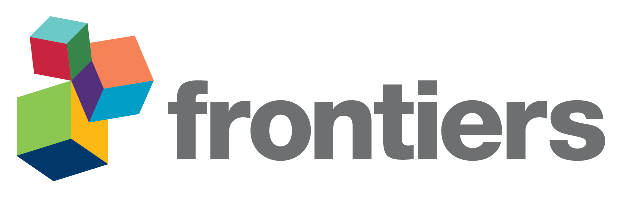
\includegraphics[width=10cm]{logo1}% This is a *.eps file
%\end{center}
%\caption{ Enter the caption for your figure here.  Repeat as  necessary for each of your figures}\label{fig:1}
%\end{figure}


\bibliographystyle{frontiersinSCNS_ENG_HUMS} % for Science, Engineering and Humanities and Social Sciences articles, for Humanities and Social Sciences articles please include page numbers in the in-text citations
%\bibliographystyle{frontiersinHLTH&FPHY} % for Health, Physics and Mathematics articles
\bibliography{../ref/UEH-EVN-Data}

\end{document}
